\chapter{Optimal Calibrations}
\section{General} % FIXME: the sections structure should be re-arranged/intergrated into the main general structure (the Introduction.tex part was untouched)

%% General
% From NGT Proposal: 
% This task will optimize the calibration process for the CMS detectors, from hours currently, to an online predictive model leveraging AI techniques. Such an improvement is essential to push real-time analysis based on R3 software (task 3.1) to the same accuracy that we typically achieve offline. One could then store high-quality high-level information, which implies a big save in terms of storage.

% Deliverable/milestone: Production of a report illustrating the current calibration workflows in CMS and evaluating the impact of non-optimal calibrations on the physics performance of the online reconstruction.

\begin{figure}[h!]	
\centering
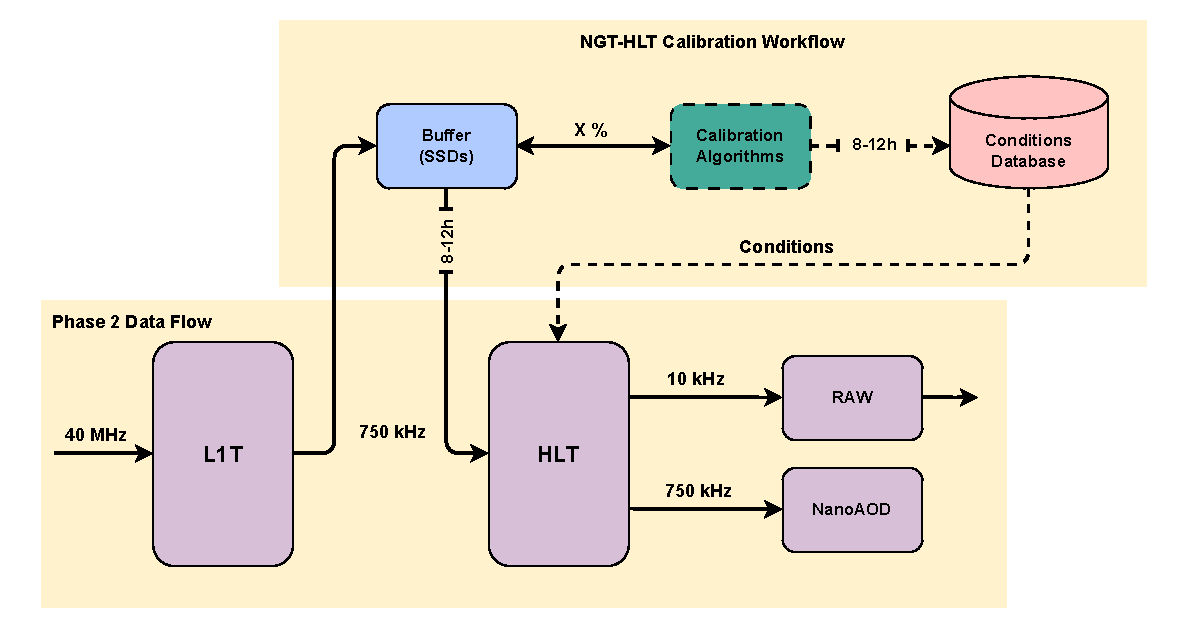
\includegraphics[width=\textwidth]{figures/NGT-HLT_Calibration_Workflow.pdf} %\hfill
\caption{Conceptual Design of $\mathrm{R}^{3}$ Optimal Calibrations (NGT-HLT Calibration Workflow)}
\label{fig:NGT-HLT_CalibrationWorkflow}
\end{figure}

\section{Calibration Workflows Analysis}
% Conduct a comprehensive analysis of the current calibration workflows and procedures within CMS currently in place, understanding the intricacies of the process, and identify areas for improvement (bottlenecks) in the calibration process. 

% NOTE: The current preliminary survey focused on finding viable candidates for the prototype. A continued and more detailed follow-up survey is being planned, especially in the context of Phase 2 calibrations, including new detectors (MTD, HGCAL, new tracker, etc.)

%\subsection{CMS Calibration Workflows}
% TODO: General introduction

% TODO: explain general AlCa: calibration vs condition, records, tags, etc.

% Latest GTs:
326 conditions (records/tags) in the latest HLT Global Tag (\texttt{140X\_dataRun3\_HLT\_v3}) used during LHC Run 3 p-p data taking in 2024.

% NOTE: Introduce prompt/offline in a similar manner?

\subsubsection{PCL}
\subsubsection{O2O}

⁄⁄‹\subsubsection{Other}
\subsection{Pixel Tracker Calibrations}

The CMS SiPixel detector is integral to the High-Level Trigger (HLT) decision-making process. This part of the report delves into the calibration prospects of the SiPixel detector, emphasizing unused records, FED cabling, gain and quality calibrations, CPE conditions, and alignment practices. Future prospects and recommendations for improving calibration workflows under the NGT framework are also discussed.
Out of the 326 conditions in the HLT GT, 13 are related to the Silicon Pixel Tracker, of which 12 are relevant to Run 3 data-taking. From these, the following 8 are considered core and critical for data-taking:

\begin{table}[h!]
    \centering
    \begin{adjustbox}{max width=\textwidth}
    \begin{tabular}{p{3.5cm}|p{4cm}|p{2.5cm}|p{2cm}|p{4.5cm}}
        \textbf{Name} & \textbf{Record} & \textbf{Workflow} & \textbf{Frequency of Updates} & \textbf{Description} \\ \hline
    \end{tabular}
    \end{adjustbox}
    \caption{Fundamental Silicon Strip Tracker Calibrations, ordered in terms of frequency of updates.}
    \label{tab:PixelCalibrations_critical}
\end{table}

\subsubsection{Unused Records in SiPixel Calibration}
Several records remain unused at HLT but hold relevance for other operational aspects:
\begin{itemize}
    \item \texttt{SiPixelDetVOffRcd}: Lists detector IDs with HV or LV off. Payload is ideal or empty.
    \item \texttt{SiPixelGainCalibrationOfflineRcd}: Stores gain and pedestal values for offline analysis.
    \item \texttt{SiPixelLorentzAngleRcd ("from alignment")}: Contains Lorentz Angle offsets, outdated since 2017.
    \item \texttt{SiPixelTemplateDBObjectRcd ("0T")}: Used during 0T templated tracking for PixelRecHits.
\end{itemize}

\subsubsection{FED Cabling and Calibration Maps}
The \texttt{SiPixelFedCablingMapRcd} records cabling maps connecting FEDs to readout channels. While not a direct calibration, this record plays a vital role in detector topology and reconstruction. This was last updated in 2017 with the transition to the Pixel Phase-1 detector.

\subsubsection{Bad components}
Description: This payload contains the DetIDs and ROCs associated with those DetIDs that are considered "dead." Used by tracking.\\
Record Name: \texttt{SiPixelQualityRcd} 

\subsubsection{Pixel Lorentz Angle}
Description: The 'no label' payload contains the value of LorentzAngle / Tesla for the Barrel Pixel and Forward Pixel separately (due to different HV constants, geometry, etc.).\\
Record Name: \texttt{SiPixelLorentzAngleRcd} 
Labels = none, \texttt{fromAlignment} or \texttt{forWidth} - given when included in a global tag.
\begin{itemize}
\item \texttt{fromAlignment} : the LA offset generated by alignment (alternative to LA correction from templates).
\item \texttt{forWidth}: the LA for charge width estimate in the generic CPE (alternative to the same LA as for offset). 
\end{itemize}

\subsubsection{Pixel Templates}
Description: used in the templated tracking algorithm for Pixel RecHits.
Record Name:  \texttt{SiPixelTemplateDBObjectRcd} 

\subsubsection{Generic Errors}

Description: used in the generic CPE (cluster position estimation) algorithm as errors. Improves irradiation bias corrections (IBC) for data.
Record Name:  \texttt{SiPixelGenErrorDBObjectRcd}

\subsubsection{Pixel Alignment}
Records used: 
\begin{itemize}
\item \texttt{TrackerAlignmentErrorRcd} (for alignment), 
\item \texttt{TrackerSurfaceDeformationRcd} (for surface deformation)  \item \texttt{GlobalPositonRcd} (defining the relative position of the subdetectors) 
\end{itemize}

Tracker alignment is tightly coupled with CPE conditions to mitigate Lorentz Angle miscalibrations. High-granularity offline PCL helps optimize biases but is prone to weak modes.
HLT reconstruction uses the Pixel CPE Fast algorithm (a variant of the generic algorithm), while offline operations rely on Pixel Template reconstruction. Discrepancies between these algorithms necessitate customized alignment procedures.

\begin{figure}[htbp]
   \centering
	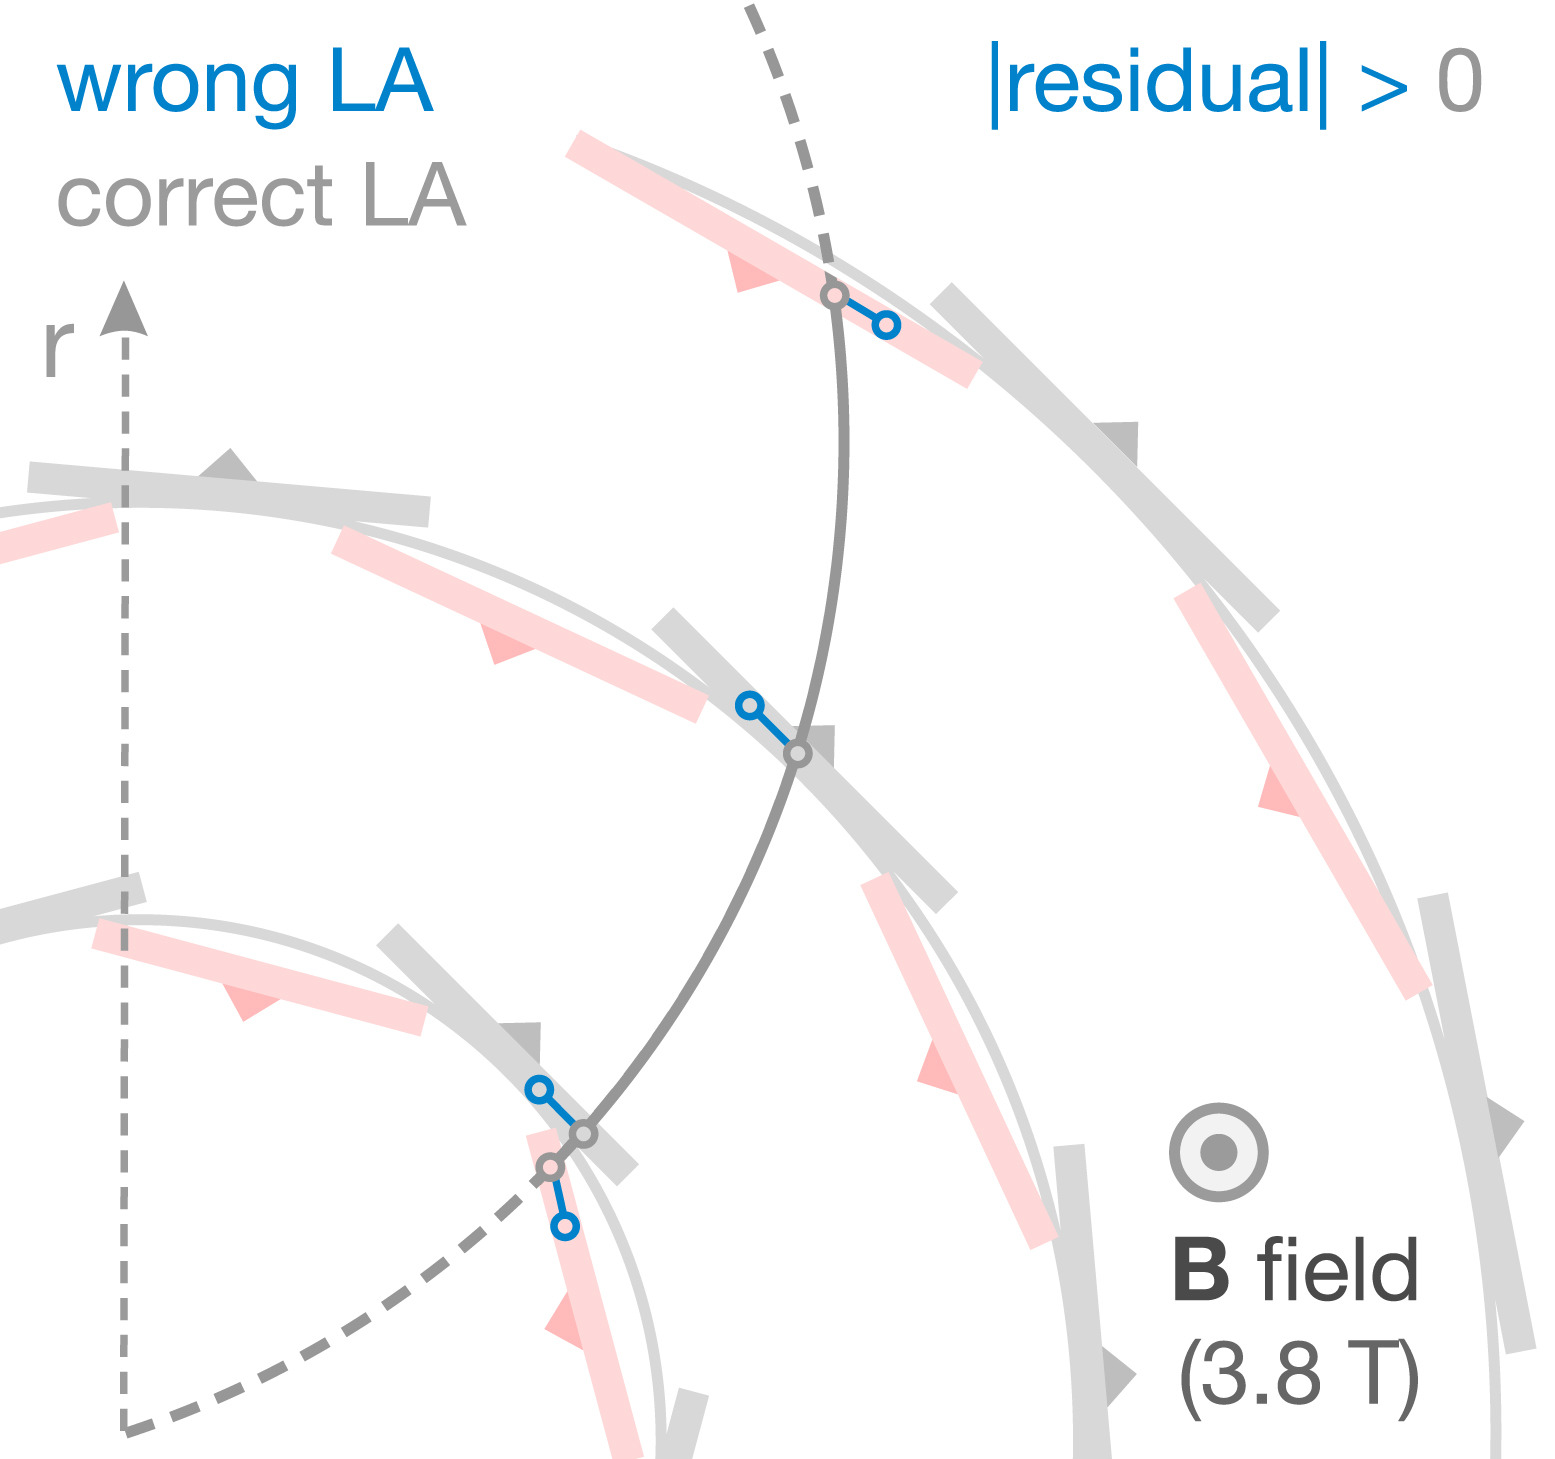
\includegraphics[width=0.5\textwidth]{figures/pixel_alignment_sketch.png}
   \caption{Sketch showing the transverse view of the Phase-0 barrel pixel subdetector, made of successive layers of silicon modules. The alternating orientation of the modules within each layer is indicated by the triangles. The blue (grey) circles represent the reconstructed hit positions using incorrect (correct) Lorentz angles in the presence of a magnetic field . The grey curve corresponds to a track built from the hits that were reconstructed with the correct Lorentz angles. Hits reconstructed with incorrect Lorentz angles are displaced in a direction defined by the orientation of the module, increasing the residual distance between the hits and the track. \cite{CMS:2022ali}}
   \label{fig:pixelAlignment}
\end{figure}

\subsubsection*{Future Prospects and Integration in NGT Demonstrator Workflow}
\begin{itemize}
    \item \textbf{Bad Components Masking}:
    \begin{itemize}
        \item Already implemented in PCL workflows and requires minimal statistics for updates.
        \item Demonstrated to improve track building in inside-out muon reconstruction.
    \end{itemize}
    \item \textbf{Pixel Alignment}:
    \begin{itemize}
        \item Enhancing alignment directly impacts B-tagging and physics trigger performance.
        \item Requires tailored workflows to address weak modes effectively.
    \end{itemize}
\end{itemize}

\subsubsection*{Recommendations}
\begin{itemize}
    \item Prioritize the inclusion of bad components masking in the NGT demonstrator workflow due to its operational simplicity and demonstrated impact.
    \item Develop alignment calibration workflows that directly integrate HLT tracks to ensure compatibility.
    \item Evaluate the feasibility of frequent updates for gains and CPE conditions to maintain precision.
\end{itemize} % Marco
\subsection{Strip Tracker Calibrations}

Out of the 326 conditions in the HLT GT, 24 are related to the Silicon Strip Tracker, of which 21 are relevant to Run 3 data-taking. From these, the following 4 are considered core and critical for data-taking:

\begin{table}[h!]
    \centering
    \begin{adjustbox}{max width=\textwidth}
    \begin{tabular}{p{3.5cm}|p{4cm}|p{2.5cm}|p{2cm}|p{4.5cm}}
        \textbf{Name} & \textbf{Record} & \textbf{Workflow} & \textbf{Frequency of Updates} & \textbf{Description} \\ \hline
    \end{tabular}
    \end{adjustbox}
    \caption{Fundamental SiStrip Calibrations, ordered in terms of frequency of updates.}
    \label{tab:StripCalibrations_critical}
\end{table}

\subsubsection{DAQ O2O conditions}

\subsubsection{DCS O2O conditions}

\subsubsection{Bad Components}

\subsubsection{APV gains}

\subsubsection{CPE conditions}

\subsection{Others} % Marco
%%!TEX root = ../main.tex
\subsection{ECAL Calibrations}

%%% I don't know how much I believe these numbers here.
Out of the 326 conditions in the HLT GT,
67 are related to ECAL, %59 
of which 52 are relevant to \Runthree data-taking. %36
From these, the following are considered core and critical for data-taking:
\begin{table}[h!]
    \centering
    \begin{adjustbox}{max width=\textwidth}
    \begin{tabular}{p{3.5cm}|p{4.5cm}|p{2.5cm}|p{2cm}|p{4cm}}
        \textbf{Name} & \textbf{Record} & \textbf{Workflow} & \textbf{Frequency of Updates} & \textbf{Description} \\ \hline
    Laser corrections & \texttt{EcalLaserAPDPNRatios} & ECAL automation and manual & Every 40 min or per fill & Crystal transparency and photodetector response. \\
    Pedestals & \texttt{EcalPedestals} & PCL and ECAL automation & Per run or weekly & Pedestals for noise measurements. \\
    Pulse shapes & \texttt{EcalLaserAPDPNRatios} & ECAL automation and manual & 3 days & Pulse shapes. \\
    Timing & \texttt{EcalTimeCalibConstants} & ECAL automation and manual & Weekly & Time of the pulse maximum.\\
    Intercalibrations & \texttt{EcalIntercalibConstants} & ECAL automation and manual & Weekly or more & Equalise crystal response vs. $\eta$ and $\phi$.
    \end{tabular}
    \end{adjustbox}
    \caption{Fundamental ECAL Calibrations, ordered in terms of frequency of updates.}
    \label{tab:ECALCalibrations_critical}
\end{table}

\subsubsection{Pedestals}

%EcalPedestalsRcd

The ECAL pedestals represent the baseline from which the electronics pulses are measured.
Pedestals are measured for the three possible configurations (gains) of the multi-gain preamplifier integrated in the ECAL readout chip: $\times 1$, $\times 6$ and $\times 12$.
In the offline tag, 
the PCL updates the G12 pedestals automatically, while
the G1 and G6 pedestals are updated manually every week.
In the online tag, all three pedestals are updated manually weekly.

\subsubsection{Laser Corrections}

%EcalLaserAPDPNRatiosRcd

The transparency of the ECAL crystals and the photodetector's response to light are degraded as an effect of the irradiation from the LHC collisions.
The degradation as a function of time is monitored crystal by crystal by measuring the response to the light of a laser system.
The light is injected in the system during the LHC abort gap, and a complete scan of the calorimeter takes 40 minutes.
The measurement of the response degradation is then used as a correction factor in the energy reconstruction.
In the offline tag, this correction is available with that same 40-minutes granularity,
while in the online tag it is available only once per LHC fill.

\subsubsection{Pulse Shapes}

%EcalPulseShapesRcd

The ECAL pulse shapes also change because of the irradiation affects,
and those changes also directly change the reconstruction of the signal amplitude.
These updated are more critical after a technical stop of the LHC.
The same payloads are used in the offline and online tags.

\subsubsection{Timing Corrections}

%EcalTimeCalibConstantsRcd

The ECAL timing drifts 
towards negative times during collisions 
and
towards positive times during recovery.
For the current standard used for the calibration (ratio timing), 
the same payloads are used in the offline and online tags.

\subsubsection{Intercalibrations}

%EcalIntercalibConstantsRcd

The intercalibrations are derived for each crystal and employ a series of methods:
the azimuthal symmetry of the energy deposits in ECAL,
the known mass of particles that decay to electrons and photons
($\text{Z}\to\text{ee}$, $\pi^0\to\gamma\gamma$),
and
the energy--momentum ratio ($E/p$) of electrons from electroweak boson decays.
In general these calibrations require multiple inverse femtobarns of integrated luminosity to derive;
the same payloads are used in the offline and online tags.

\subsubsection{Alignment}

Alignment of the ECAL with respect to the Tracker system is done infrequently, 
mainly when there is a cycle of the CMS magnet.

In view of the above discussion, we consider the \emph{laser corrections} a possible candidate for the implementation in NGT.
The gap between online and offline update frequencies (40 minutes vs. per fill) is large enough that, in principle, expressive improvements can be realised by improving the online calibration. % Thiago
\subsection{HCAL Calibrations}

The calibration of the hadron calorimeter\footnote{Details of the detector are presented in \ref{CMS}} (HCAL) is vital in the determination of the energy scale and resolution of hadrons, and consequently jets and missing transverse momentum.

There are no HCAL calibrations included in the PCL, however, there exist HCAL automation workflows that update HCAL conditions on a weekly basis (e.g. gains, pedestals). Most conditions are explicitly baked into the Look-Up Tables (LUTs) that are loaded on-detector and append the GT via the O2O procedure semi-automatically. The remaining conditions are uploaded manually to the conditions database. Many HCAL conditions are also relevant for L1T and the corresponding trigger primitives. Out of the 326 conditions in the HLT GT, 37 are related to HCAL, of which 24 are relevant to Run 3 data-taking. From these, the following 9 are considered core and critical for data-taking:

\begin{table}[h!]
    \centering
    \begin{adjustbox}{max width=\textwidth}
    \begin{tabular}{p{3.5cm}|p{4cm}|p{2.5cm}|p{2cm}|p{4.5cm}}
        \textbf{Name} & \textbf{Record} & \textbf{Workflow} & \textbf{Frequency of Updates} & \textbf{Description} \\ \hline
        Gains (RadDam) & \texttt{HcalGains} & O2O & Weekly & Response corrections for radiation damage (RadDam). \\
         Pedestals & \texttt{HcalPedestals} & HCAL automation (O2O) & Weekly & Pedestals for noise measurements.
measurements.\\
        Pedestal Widths & \texttt{HcalPedestalWidths} & HCAL automation (O2O) & Weekly & Pedestals for noise measurements.
measurements. \\
        L1T Trigger Objects & \texttt{HcalL1TriggerObjects} & HCAL automation (O2O) & Weekly & L1T trigger objects, including relevant conditions: pedestals, gains and response corrections, channel quality. \\
        Response Corrections & \texttt{HcalRespCorrs} & O2O & per Era ($\approx 20~\fbinv$) & Corrections to detector energy response. \\
        Channel Quality & \texttt{HcalChannelQuality} & O2O & Few times per year & Tracking dead or non-functional HCAL cells. \\
        Geometry Parameters & \texttt{HcalParameters} & Manual & Yearly & Parameters related to the HCAL geometry. \\
        Look-Up Tables (LUTs) & \texttt{HcalLUTCorrs} & O2O & Rarely & Corrections related to Look-Up Tables (LUTs). \\
    \end{tabular}
    \end{adjustbox}
    \caption{Fundamental HCAL Calibrations, ordered in terms of frequency of updates.}
    \label{tab:HCALCalibrations_critical}
\end{table}

In the context of an optimal calibrations workflow, the first 6 from Table \ref{tab:HCALCalibrations_critical} are considered fundamental\footnote{There exist fundamental HCAL conditions or calibrations which can have a significant effect on HLT reconstruction that are implemented in the hardware directly (e.g. timing alignment, zero-suppression thresholds, \texttt{HcalZSThresholds}) while their conditions database records may not be considered critical per se (but rather used for bookkeeping purposes).} and generally require more frequent updates. These have been analysed in more detail in the following sections. % NOTE: footnote could be moved to Others section.

\subsubsection{Response Corrections}
Response corrections are calibrations that aim to equalise the signal coming from the detector to provide a uniform energy measurement. They have a very significant effect on HLT reconstruction and rates, and thus are considered critical. Generally, they are updated roughly every era ($\approx 20 \fbinv$), however, the exact frequency depends on the HCAL subsystem and type of correction. Generally, the required statistics determines the frequency, as the analyses are often statistically limited. Technically-speaking, if the calibrations are determined accurately, they would require less-frequent updates (modulo hardware changes). The updates are explicitly baked into the LUTs that are loaded on-detector and the corresponding conditions appended to HLT GT via the O2O procedure semi-automatically.

% HB and HE
The main calibrations for the HB and HE come in in two forms: azimuthal ($\phi$\texttt{-symmetry}) and isolated track (\texttt{IsoTrack}) corrections, which are multiplicative factors. 

% Azimuthal (Phi-)Symmetry
Asymmetries in the response over $\phi$ arise due to structure, materials, inhomogeneous magnetic field, beam-spot shifts, and miscalibrations. The $\phi$\texttt{-symmetry} intercalibrations equalize the detector response in $\phi$ for each $i\eta$ ring and depth section of the HCAL. They take advantage of the uniformity of particle energies across the azimuthal angle $\phi$. An intercalibration is performed between calorimeter channels by comparing it to the average collected energy in the entire $i\eta$ ring. Two methods are used to determine them, depending on the hadron energies:
\begin{itemize}
    \item For high energies ($> 4 \GeV$) an iterative method is used, where scale factors for uncalibrated energies are determined iteratively by equalizing the mean of the energies in an energy interval. An unbiased dataset is used with events triggered by detectors other than HCAL, such as electron, photon and muon triggers. The reconstructed energies are obtained from zero-suppressed events after noise (pedestal) subtraction.
    \item For low energies ($< 4 \GeV$; down to a fraction of a GeV), a method of moments is used, where the first (mean) and second (variance) moments of the energy distribution are compared to that of the entire $i\eta$ ring. This method uses minimum-bias events taken without zero-suppression (NZS). The noise (pedestal) is subtracted from the energy distribution.
\end{itemize}

The uncertainty-weighted average of the scale factors from both methods is used as the final scale factor for the $\phi$-intercalibration.

% Isolated Track (IsoTrack)
An absolute calibration of charged hadrons is performed by comparing the energy measurement with that of the tracker system, taking advantage of the precise calibration of the tracker system. Unlike the tracker momentum measurement, the HCAL energy response is non-linear, especially at lower energies. Therefore, the goal of the calibration is to equalize the relative energy scale for higher momentum charged hadrons that do not interact hadronically with the ECAL. Isolated tracks of hadrons with momenta between $40-60 \GeV$ are used. Data samples are collected using dedicated \texttt{IsoTrack} triggers with special isolation and maximum requirements on the energy deposited in the ECAL, as well as a more standard set of physics triggers with similar selections applied offline. Assuming there are no statistical limitations, preferably they are determined in a depth-dependent way, which is more optimal.

% HF
The forward calorimeter (HF) is also calibrated using the $\phi$-symmetry, while the energy scale is extrapolated using $Z \rightarrow ee$ events. The dataset consists of events with one electron candidate in the HF and the other in the ECAL, which has been precisely calibrated. The scale is adjusted so that the dielectron invariant mass corresponding to the Z-peak is consistent between data and simulation.

% HO, ZDC
For HO, the intercalibration makes use of muons from collision data, as well as cosmic ray muons, while the determination of the absolute energy scale makes use of di-jet events. These calibrations are mostly unchanged with respect to initial calibrations.

The Zero-Degree Calorimeter (ZDC) calibrations are also mostly unchanged and are not discussed here further. 

% NGT candidate assessment
In the context of a potential candidate for the optimal NGT calibrations, it is clear that the response corrections involve a number of dedicated separate offline analyses for different HCAL subsystems, using various input datasets (incl. \texttt{AlCaRecos}) and specific selections. Thus, their determination is rather convoluted and they are tricky to do without proper offline analysis and corresponding validation. Even though some of the sub-calibrations might be reasonably possible to automate (e.g. $Z \rightarrow ee$ for HF), it would still require significant work to automate. Furthermore, since they are baked into the LUTs, they are entangled together with L1T condition updates. Therefore, one can conclude that the response corrections are not a viable candidate for the NGT workflow in their current form, especially for the Run 3 prototype.

\subsubsection{Gains (RadDam)}\label{sec:HCAL_gains}
The  \textit{gains} (or \texttt{RadDam}) calibrations are responsible for correcting for radiation damage in the HCAL. Generally this leads to a decreased signal due to the darkening of active scintillator material and fibres (similar to the ECAL laser corrections covered in Section \ref{sec:ECALlaser}). Conversely, the recovery process of thermal annealing also effects the signal and needs to be corrected for. Due to the increased radiation in the forward region, primarily HE and HF are corrected. These corrections are especially important in the high $|i\eta|$ regions where there is no tracker coverage and the \texttt{IsoTrack} response corrections are less accurate and cannot cover for these differences. Therefore, they can be considered critical especially for those regions. HB and HO have not been corrected for a long time due to lower radiation damage. The corrections are determined $|i\eta|$- and depth-dependent and $|i\phi|$-independent) yielding a multiplicative factor together with the response corrections for final calibrated response in GeV. Generally, they are updated via the O2O procedure semi-automatically (as with the response corrections) roughly every era ($\approx 20 \fbinv$).

Typically, the measurements of the radiation damage is based on laser data in the orbit/abort gap, when there is no beam in the LHC. The laser system sends light to the photodetectors (SiPMs, PMTs) or directly to the scintillators. The ratio of the amplitudes gives a measure of the signal attenuation. The laser data is then compared to that taken at the start of the yearly data-taking in order to measure the net effects of radiation damage. A new dedicated radiation damage monitoring system was recently developed for the HF quartz fibres. 

The effects of radiation damage are dependent on the delivered luminosity. The dependence is modelled and parametrised to exponential decay \cite{CMS-PRF-18-003}. An example of the relative laser signal in a single $i\eta$ region and layer is shown in Figure \ref{fig:ECAL-Laser_data}. 

\begin{figure}[h!]	
\centering
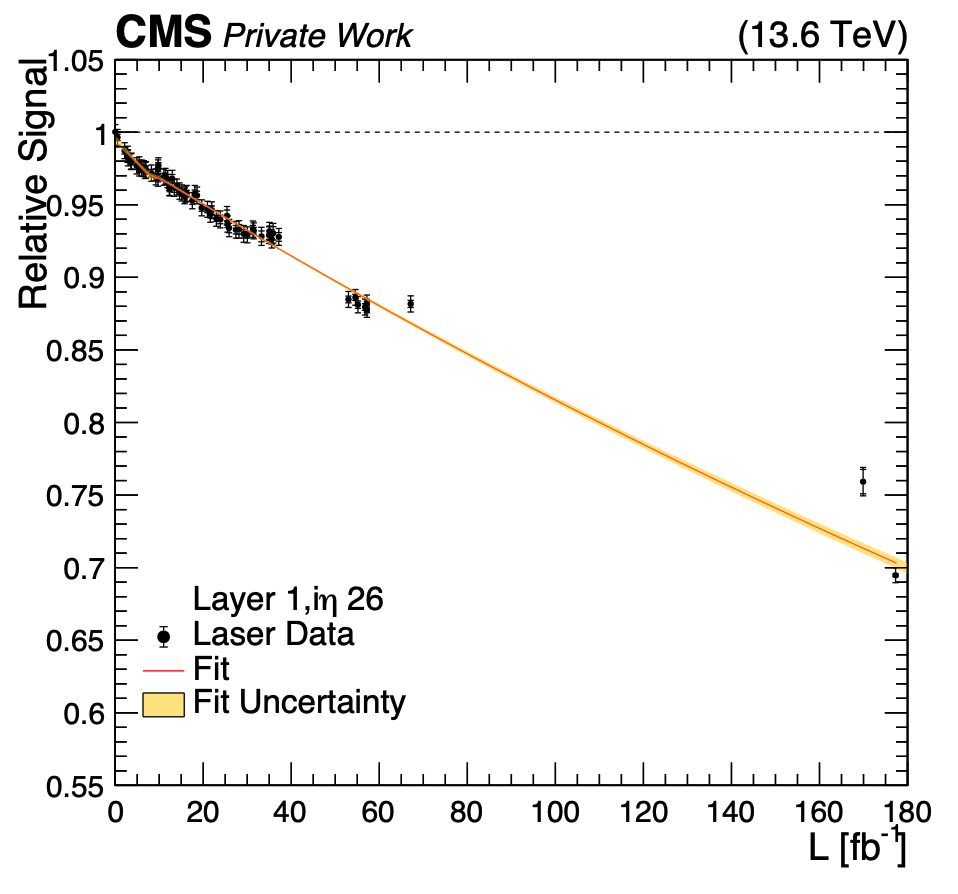
\includegraphics[width=0.7\textwidth]{figures/HCAL-Laser_data2024.png} %\hfill
\caption{Laser system data in layer 1, $i\eta = 27$ of the HCAL, indicating the relative signal as a function of the total integrated luminosity L in $\fbinv$, parametrised as exponential decay. The missing data points indicate the extended downtime of the laser system in 2024.}
\label{fig:HCAL-Laser_data}
\end{figure}

In the case of downtime of the laser system (also seen in Figure \ref{fig:ECAL-Laser_data} for 2024), the backup approach are dedicated energy flow extrapolations, which are non-trivial. Therefore, the preference is to use laser data.

% NGT candidate assessment
In the context of a potential candidate for the optimal NGT calibrations, the gains or \texttt{RadDam} corrections are important for HLT reconstruction and require frequent updates. There are plans to include them in the HCAL automation system (covered in more details the next Section \ref{sec:HCAL_pedestals}) within weekly updates. Therefore, they are a good candidate for the NGT workflow. One caveat is that they are dependent on laser data, which requires different data stream than the standard bulk collisions data. Furthermore, a vital requirement is a well-functioning laser system.

\subsubsection{Pedestals}\label{sec:HCAL_pedestals}
The HCAL pedestals and their corresponding widths are essentially measurements of the noise "floor" that are offset to avoid any energy measurement bias. Generally-speaking, noise increases with radiation damage. Regular pedestal updates are important to avoid any drifting of HCAL-driven trigger rates and contributions to the fraction of the energy deposited in the HCAL and ECAL, $\frac{H}{E}$, which is an observable used in the identification of electrons and photons, including shower shapes and isolation. The pedestals are also important inputs into other calibrations, such as the response corrections.

Generally, they are updated roughly every week ($\approx 2 \fbinv$), as part of the HCAL automation workflow. The workflow is used to calculate effective pedestals from collision runs, where good input data from candidate runs is identified and processed within 1 hour after a given LHC fill. The input data is based on measurements in orbit/abort gap when there is no beam in the LHC (similarly to the laser data for the HCAL gains discussed in the previous Section \ref{sec:HCAL_gains}). The conditions are automatically uploaded to the conditions database via the O2O procedure. Validation in the context of changes to L1T and HLT trigger rates are produced within 2 hours, with an ultimate validation and green-light from AlCa typically after 1-2 days. Given a successful validation, this is followed by deployment at the subsequent LHC interfill period.

% NGT candidate assessment
In the context of a potential candidate for the optimal NGT calibrations, the pedestals are critical inputs. The are included in the HCAL automation system within weekly updates, which automatically make them a good candidate for the NGT workflow. One caveat is that they are dependent on orbit/abort gap data, which requires different data stream than the standard bulk collisions data.

% \subsubsection{Others}

% NOTE: more complete list in annex? e.g. non-critical calibrations % Mateusz
%%!TEX root = ../main.tex
\subsection{Muons System Calibrations}

Out of the 326 conditions in the HLT GT,
41 are related to the muon systems:
14 to the Drift Tubes (DTs),
20 to the Cathode Strip Chambers (CSCs),
and
7 to the Resistive Plate Chambers (RPCs).
No conditions are related to the Gas Electron Multipliers (GEMs) as of 2024,
and
the RPCs don't have calibrations that can affect the data quality.
The only conditions that are considered core for data-taking are:
\begin{table}[h!]
    \centering
    \begin{adjustbox}{max width=\textwidth}
    \begin{tabular}{p{3.5cm}|p{4.5cm}|p{2.5cm}|p{2cm}|p{4cm}}
        \textbf{Name} & \textbf{Record} & \textbf{Workflow} & \textbf{Frequency of Updates} & \textbf{Description} \\ \hline
    DT drift velocity & \texttt{DTMtime} & Manual & Rarely & Drift velocity of the ionisation electrons. \\ 
    DT timing offset & \texttt{DTTtrig} & Manual & Yearly & Timing offset of the ionisation electrons. \\ 
    CSC time corrections 	& \texttt{CSCChamberTimeCorrections} & Manual & Yearly & Adjustments to center reco. hit times at $t=0$. \\
    						& \texttt{CSCDBChipSpeed} & Manual & Rarely & \\ 
	CSC electronics & \texttt{CSCDBGains} & Manual & Yearly & Electronics parameters of strips channels. \\
                    & \texttt{CSCDBPedestals} & Manual & Yearly &  \\
					& \texttt{CSCDBCrosstalk} & Manual & Yearly &  \\ 
                    & \texttt{CSCDBNoiseMatrix} & Manual & Yearly &  \\
    \end{tabular}
    \end{adjustbox}
    \caption{Fundamental Muon System Calibrations, ordered in terms of frequency of updates.}
    \label{tab:MuonCalibrations_critical}
\end{table}

In all conditions related to the muon systems, all workflows are manual, the frequency of updates is small, and payloads are always kept the same between online and offline.
As such, we conclude that the muon system doesn't provide any candidate conditions for the NGT project.
 % Thiago

\section{Physics Performance}

%%% Here we discuss the 
%% Physics performance
% Assessment on the impact of non-optimal calibrations on the physics performance of the online reconstruction, by analysing data to quantify the effects of calibration inaccuracies.
